\providecommand{\pdfxopts}{a-1b,cyrxmp}
%\providecommand{\pdfxopts}{a-1b}
\providecommand{\thisyear}{2021}
\immediate\write18{rm \jobname.xmpdata}%  uncomment for Unix-based systems
\begin{filecontents*}{\jobname.xmpdata}
\Title{ЛЭТИ.849104.01 Э3 Иванов Петр Семёнович \textemdash\thisyear}
\Author{Иванов Петр Семёнович}
\Creator{pdfTeX + pdfx.sty with options \pdfxopts }
\Subject{Лабораторная работа №1
\sep
исследование операционного усилителя
\sep
выполнено студентом 8491 группы 
\sep
Ивановым Петром Семёновичом}
\Keywords{операционный усилитель, шаблон для лабораторной}
\CoverDisplayDate{март \thisyear}
\CoverDate{2020-03-22}
\Copyrighted{True}
\Copyright{Public Domain}
\CopyrightURL{http://github.com/trot-t}
\Creator{pdfTeX + pdfx.sty with options \pdfxopts }
\end{filecontents*}

\documentclass[russian,utf8,nocolumnxxxi,nocolumnxxxii]{eskdtext}

\pdfcompresslevel=9

\usepackage[\pdfxopts]{pdfx}[2016/03/09]
\PassOptionsToPackage{obeyspaces}{url}
\let\tldocrussian=1  % for live4ht.cfg

%
% https://tavda.net/blog/latex/
% 

\usepackage[TS1,T2A]{fontenc}
\usepackage[utf8]{inputenc}
\usepackage[english,russian]{babel}
\usepackage{tikz}                                            % для чертежей
\usepackage[european,cuteinductors,smartlabels]{circuitikz}  % для электронных схем
\usetikzlibrary{calc}

\usepackage{amsmath,amsfonts}
\usepackage{amssymb}
%\usepackage[scr]{rsfso} % буквы для алгебры множеств

\usepackage{gnuplottex}   % автоматическая вставка графиков из программ моделирования электрических схем


\usepackage{enumitem}

%%% Межстрочный интервал
\usepackage{setspace}

%% таблицы в стиле старых книг
\usepackage{booktabs} 

%% для подкладывания отдельных pdf-страниц 
\usepackage{pdfpages}

%% для кода
\usepackage{listings}

\definecolor{lightgrey}{rgb}{0.9,0.9,0.9}
\definecolor{lightblue}{rgb}{0,0,1}

\definecolor{grey}{rgb}{0.5,0.5,0.5}
\definecolor{blue}{rgb}{0,0,1}
\definecolor{violet}{rgb}{0.5,0,0.5}

\definecolor{darkred}{rgb}{0.5,0,0}
\definecolor{darkblue}{rgb}{0,0,0.5}
\definecolor{darkgreen}{rgb}{0,0.5,0}


\renewcommand{\lstlistingname}{\normalsize Листинг}
\newcommand{\listfile}[1]{\lstinputlisting{#1}}
\lstdefinelanguage{ngspice}{%
    morekeywords={control, end, endc, subckt, ends, plot, gnuplot, model, temp, ac, dc, tran, options, set},%
    morekeywords={CONTROL, END, ENDC, SUBCKT, ENDS, PLOT, GNUPLOT, MODEL, TEMP, AC, DC, TRAN, OPTIONS, SET},%
    directives={},
    comment=[l]{*},
    morecomment=[l]{;},
    morestring=[b]',
    morestring=[b]"
}[directives]
\lstset{%
  language=ngspice,%
  basicstyle=\ttfamily\scriptsize,%
  sensitive=true,%
  keywordstyle=\color{blue},%
  stringstyle=\color{darkgreen},%
  commentstyle=\color{violet},%
  directivestyle=\color{blue},
  showstringspaces=false,%
  tabsize=2,%
  frame=leftline,
  rulecolor=\color{lightblue},
  numberstyle=\tiny,
  numbers=left,
  numbersep=10pt,
  xleftmargin=20pt,
  framexleftmargin=2.5mm,
  framexleftmargin=5pt,
  framesep=15pt,
  fillcolor=\color{lightgrey},
  inputencoding=cp1251, % принимает только WINDOWS-1251 кодировку
   extendedchars=true
}

\def\No{\textnumero} % № для unix

\ESKDtitle{отчет по лабораторной работе}
\ESKDdocName{Операционный усилитель}
 
\ESKDdepartment{%
Государственное образовательное учреждение высшего профессионального образования
}
\ESKDcompany{%
<<Санкт-Петербургский государственный электротехнический университет "ЛЭТИ">> 
}
\ESKDauthor{\scalebox{0.6}[1.0]{Иванов-Петров~M.\,M.}} % "Разраб." в штампе на листе содержания
\ESKDchecker{\scalebox{0.9}[1.0]{Иванов П.С.}} % "Пров."  в штампе на листе содержания
\ESKDnormContr{Петров П.П.} % "Н. контр." в штампе на листе содержания
\ESKDapprovedBy{Сидоров С.С.}%  "Увт." в штампе на листе содержания
\ESKDdate{2021/02/23} % Дата (Год отображается на титульной странице) 
\ESKDsignature{ЛЭТИ.849121.01 Э3} % Шифр
\ESKDletter{}{У}{} % Литеры, для учебных работ используется литера У
 
\renewcommand{\ESKDtheTitleFieldX}{%
Санкт-Петербург
 
\ESKDtheYear~г.} % Шаблон для отображения в нижней части титульного листа города и года 
%\author{}
% Конец преамбулы

\begin{document}
\maketitle

% шаблон графика параболы
%\begin{tikzpicture}
%\newcommand{\xb}{-3}
%\newcommand{\xa}{3}
%\draw[thin, ->] (-6,0) -- (6,0) node[right] {$X$};
%\draw[thin, ->] (0,-6) -- (0,6) node[left] {$Y$};
%\foreach \x\xtext in {-5/-5,5/5,{\xb}/\xb,{\xa}/{\displaystyle \frac{-b+\sqrt{b^2-4ac}}{2a}}} % 
%   \draw (\x,0.1) -- (\x,-0.1) node[below] {$\xtext$};
%\draw[domain=-5:5, help lines, smooth]
%       plot ({\x},{0.2*(\x-\xa)*(\x-\xb)});
%\end{tikzpicture}

\vspace{-3cm}
\section{Индивидуальное задание}

Смоделировать работу схемы, использующей операционный усилитель. Коэффициент усиления по напряжению принять равным $30 + N$. Где $N$  -- порядковый номер студента в списке группы.

Реальный операционный усилитель выбрать из таблицы (\ref{opamp}). Взять строку с номером, совпадающим с порядковым номером в списке группы.

{\small
\begin{table}[!ht]
	\caption{операционный усилитель для индивидуального задания}
\begin{tabular}{ll|lll}
\toprule
	\No& Операционный усилитель&\No& Операционный усилитель& примечания\\
\midrule
1&ICL7652&15&LMC6062 &\\
2&LF301  &16&LT1013  &\\
3&LF353  &17&MC1458  &\\
4&LF356  &18&OP-07D  &\\
5&LF411  &19&OPA111  &\\
6&LF412  &20&OPA277  &\\
7&LF442  &21&OPA374  &\\
8&LHV870 &22&OPA411  &\\
9&LM118  &23&OPA445  &\\
10&LM324 &24&OPA511  &\\
11&LM4250&25&TLC27M2 &\\
12&LM6211&26&UA741   &\\
13&LM7341&27&UA747   &\\
14&LM741 &\\
\bottomrule
\end{tabular}
	\label{opamp}
\end{table}
}

Просьба для графиков использовать светлый цвет фона.

\subsection{Примеры использования данного шаблона}

Формула для коэффициента усиления по напряжению инвертирующего усилителя на основе идеального операционного усилителя

$$
K_U = U_\text{вых}/U_\text{вх} = -\frac{R_2}{R_1}
$$

% ГОСТ идеальный источник напряжения http://docs.cntd.ru/document/1200007058
\begin{figure}[!ht]
	\centering
\begin{circuitikz}
	% 
	\ctikzset{bipoles/vsourceam/inner plus={\tiny $+$}}  % для опции(если нужна) [american voltage source]
	\ctikzset{bipoles/vsourceam/inner minus={\tiny $-$}}
	\ctikzset{bipoles/generic/height=0.25}
	\ctikzset{bipoles/generic/width=0.6}
	\draw
        (0,0) node[op amp] (opamp) {}   % операционный усилитель
	(opamp.+) to[R,l=$R_3$,*-] ++(0,-2) node[tground] (gnd) {}  % неинвертирующий вход
	(opamp.+) to[R,l=$R_1$] ++(-2,0) to[V,l_=$V_1$] ++(0,-2) node[tground] {} 
	let \p1=(gnd), \p2=(opamp.-), \p3=(opamp.out), \p4=(opamp.+)  in          % координаты \p(\x,\y) входов и выходов     
	(opamp.-) to[resistor,l_=$R_2$]  ++(-2,0) -|++ ($(-2,{\y4-\y2})$)  
	to[V, l_=$V_2$]  ++(0,-2) node[tground] {}          % инвертирующий вход
	(opamp.-) to[short,*-] ++ (0,1.5) to[R,l=$R_4$] ++ ($(\x3,0) - (\x2,0)$)  % резистор обратной связи 
	to[short,-*] (opamp.out)  % выход                                  
	--++ (0.5,0) to[rmeterwa, t=v] ++ ($({\x3+1},\y1) - ({\x3+1},\y3)$) node[tground] {} 
	% питание усилителя
%	(opamp.up) --++(0,0.5) node[vcc] {} node[right]{\scriptsize  25\,\textnormal{V}}
%	(opamp.down) --++(0,-0.5) node[vee] {} node[right] {\scriptsize-25\,\textnormal{V}}
	%
	% отметим узлы
	(gnd) node[below]  {\scriptsize 0}
	(opamp.+) node[above] {\scriptsize 1}
	(opamp.-) node[below] {\scriptsize 2}
	(opamp.out) node[below]  {\scriptsize 3}
	({\x4-2cm},\y4) node[above] {\scriptsize 4}
	({\x2-2cm},\y2) node[above] {\scriptsize 5}
;\end{circuitikz}
	\caption{пример подключения идеального операционного усилителя}
\end{figure}

\lstset{caption={Пример подключения модели идеального ОУ в ngspice (849104.0101.cir)},label={849104.0101.cir}}
\lstinputlisting[language=ngspice,firstnumber=1]{849104.0101.win.cir}


\subsection{Выполнение задания}
Собираем схему, как указано на рис \ref{experiment1}
\begin{figure}[!ht]
	\centering
	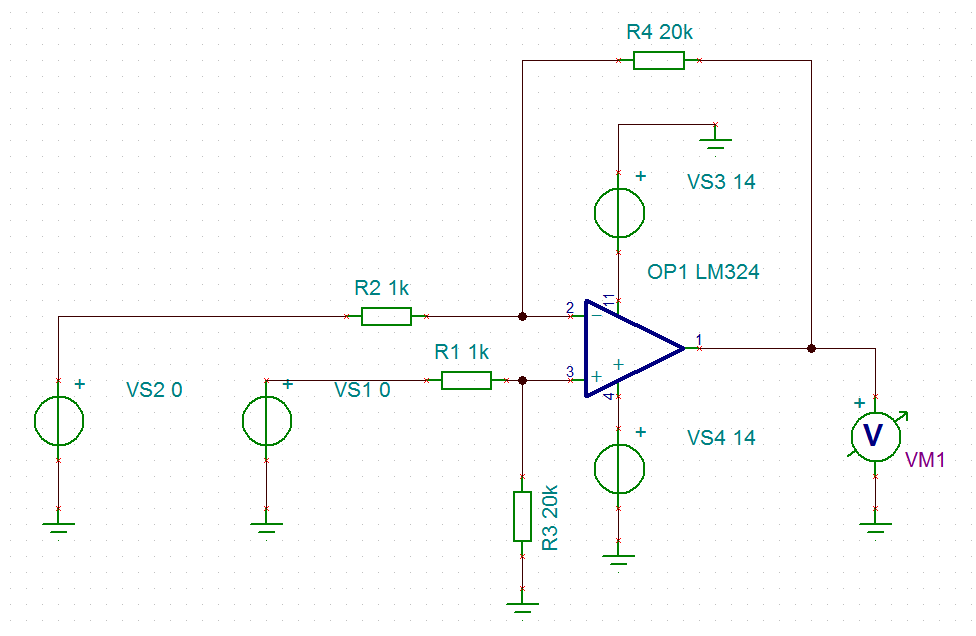
\includegraphics[scale=0.6]{schema1}
	\caption{Схема проведения опыта}
	\label{experiment1}
\end{figure}

% грязный хак
Подключение внешнего pdf-файла приведен ниже:
\newpage
\includepdf[pages={3,6}]{datchiki1.pdf}

% работа бота
\begin{figure}
	\centering
	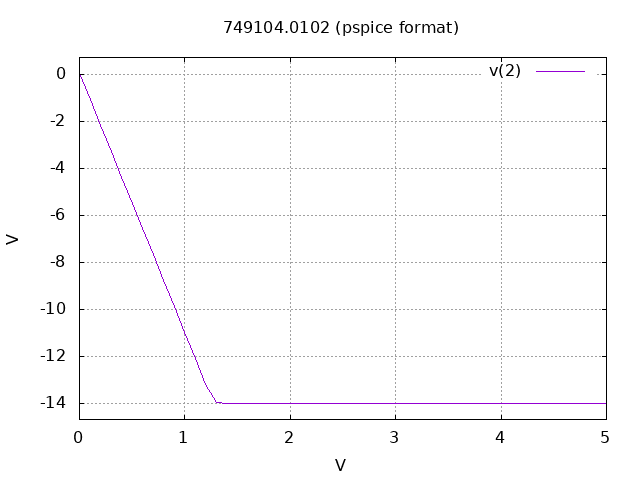
\includegraphics[scale=0.6]{749104_inv}
	\caption{пример графика зависимости выходного напряжения от входного}
\end{figure}

\lstset{caption={Пример подключения модели реального ОУ по схеме дифференциального усилителя (849124\_0224.cir)},label={849124_0224.cir}}
\lstinputlisting[language=ngspice,linerange={18-35}]{849124_0224.CIR}



\tableofcontents
%\addcontentsline{toc}{section}{Listings}
\lstlistoflistings
\end{document}
